\chapter{Basic Deployment}

\section{Deploy an EC2 instance called SSH\_gate that can be accessed via SSH from the outside world}

For this task we use an EC2 instance template that we configured with a security group that accepts SSH traffic from \texttt{0.0.0.0/0}.
To connect to the instance, we lookup the public IPv4 or domain name on the AWS web dashboard. We connect via SSH with \texttt{ssh -i [identityfile] [user]@[address]}. The identity file that belongs to our ssh-key is saved on our local machine. A list of all created ssh-keys can be seen from the dashboard, though it can only be obtained on creation. If lost, a new ssh-key must be created.


\section{Deploy an EC2 instance that hosts a web server whos purpose it is to show your name and favourite activity. This machine should only be accessible from via a SSH connection from SSH\_gate}
To create our second EC2 instance, we use a different template. It includes a new security-group that only allows SSH traffic from hosts in the security-group that we assigned to \textsl{SSH\_gate}. The exact traffic rules can be seen in Fig\ref{fig:sec_group_rules_webServer}. Furthermore, the template includes a start-up script that installs and starts a web server with a basic index.html file preloaded. We discuss this part in Section \ref{subsec:templates}.

The instance does not allow connections from SSH\_gate if we use the public IPv4. Instead we need to specify the private it IPv4 to establish a connection.
To connect to the instance, we connect first to \textsl{SSH\_gate} and use SSH from this machine to access our web server machine. Note that in order to access the web server machine, we first need to copy the identity file that is needed to authenticate the SSH session to our \textsl{SSH\_gate} machine. With that done, we can use the same command (with the new id-file) to connect to our web server EC2 instance.

Since we specified a start-up script in the template, the web server is already installed and running. We can access it in any browser under its public IPv4 address or domain name.

\section{Automatisation}

AWS offers some tools to make automatic deployment of instances with certain preferences or configurations a one-click operation. We will discuss some of the options in this section.

\subsection*{Security Groups}
Security groups allow to configure firewall like network traffic rules. A useful feature of security groups comes in the form of group referencing.\\
Since we are not assigned static IPv4/v6 addresses it would not be possible to set up general-purpose rules that can be applied to instance types. With group referencing, we can tell an instance to only accept traffic from one (ore more) of our other security groups.\\
\\
In this assignment we use security groups to make sure our second EC2 instance that hosts the web server can only be accessed via SSH form our \textsl{SSH\_gate} instance, but will allow \texttt{http} from the internet.
In Fig \ref{fig:sec_group_rules_webServer} we show the in- and out-bound rules we configured for the EC2 instance that is supposed to host the web server and should only be accessible vie SSH from our \textsl{SSH\_gate} EC2 instance.

\begin{figure}
	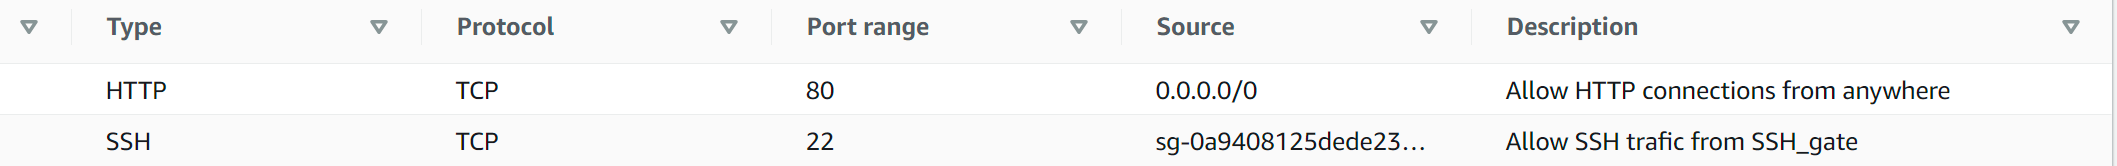
\includegraphics[width=\linewidth]{figures/webserver_sec_group_inbound.png}
	\caption{In-bond rules for security-group \texttt{webServer}}
	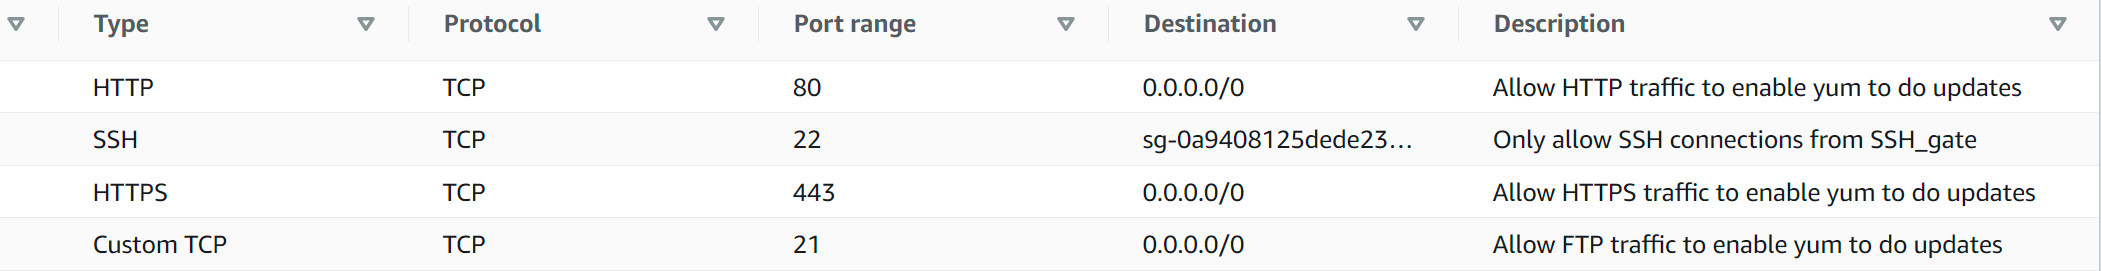
\includegraphics[width=\linewidth]{figures/webserver_sec_group_outbound.png}
	\caption{Out-bond rules for security-group \texttt{webServer}}
	\label{fig:sec_group_rules_webServer}
\end{figure}


\subsection*{Instance Launch Templates}
\label{subsec:templates}
This feature of AWS allows to save launch configurations for our EC2 instances. In addition to basic, static configurations such as ssh-keys to use, it allows us to define scripts to run one on start-up of the instance to configure the machine on OS level.\\
\\
For our WebServer instance template we use the following script to install and launch a basic web server with a page that states name and favourite activity:
\begin{lstlisting}
#!/bin/bash
yum update -y
yum -y install httpd
systemctl enable httpd
systemctl start httpd
echo '<<!DOCTYPE html>
<html>
<head>
<title>My Name and Interests</title>
<style>
/* CSS styling for the text */
body {
	font-family: Arial, sans-serif;
	text-align: center;
	background-color: #f0f0f0;
}

h1 {
	color: #333;
}

p {
	color: #666;
}
</style>
</head>
<body>
<h1>My name is <span style="color: #007bff;">Karl</span></h1>
<p>I like to go <span style="font-weight: bold;">sailing</span>.</p>
</body>
</html>
>' > /var/www/html/index.html
\end{lstlisting}

\section{Architechtural Diagram}

In this part we describe the architectural layout of the deployed AWS configuration. In Fig. \ref{fig:architechture_AWS_config} we depict the the allowed traffic between our three network nodes. In this case, the node called \textsl{Internet} refers to any user from the subnet \texttt{0.0.0.0/0}, though only a user with the IDfile for \textsl{SSH\_gate} may access that machine via SSH, while any user may access the web server via standard \texttt{http} protocol.

The machine that hosts the web server may only be accessed via SSH (for configuration purposes) from inside the AWS, thus the private IPv4 that is used inside AWS has to be used to access the machine. The security-group will block all inbound SSH traffic that does not originate from an IP address affiliated with EC2 instances that are assigned the \textsl{SSH\_gate} security-group. This way, we do not have to set the (volatile) IP address manually every time we start up the instances from the top.
The web server instance will allow \textsl{http} requests from every IP in the Internet in order to be accessible to users all over the world.
\begin{figure}[h!]
\begin{center}
	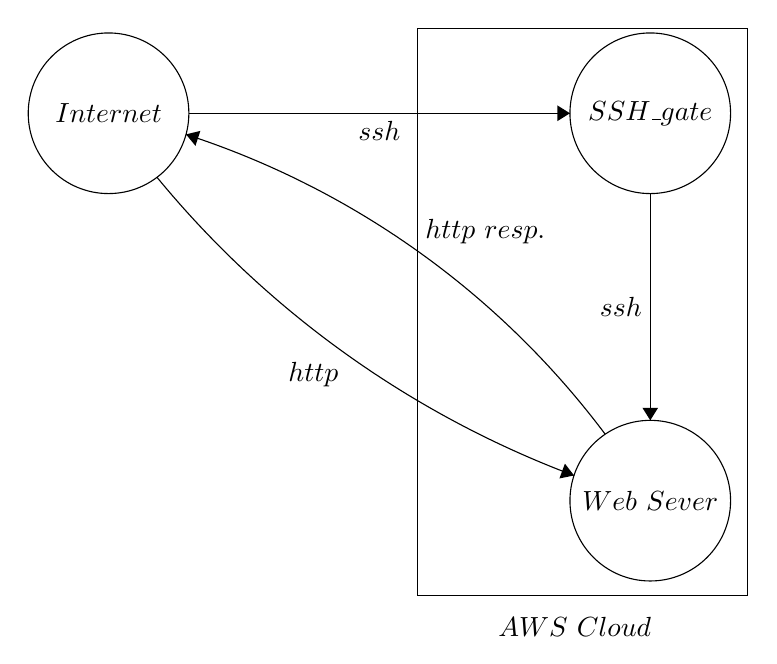
\begin{tikzpicture}[scale=0.2]
		\tikzstyle{every node}+=[inner sep=0pt]
		\draw [black] (5.4,-5.4) circle (5.1);
		\draw (5.4,-5.4) node {$Internet$};
		\draw [black] (46,-36) rectangle (25, 0);
		\draw (35,-38) node {$AWS\mbox{ }Cloud$};
		\draw [black] (39.8,-5.4) circle (5.1);
		\draw (39.8,-5.4) node {$SSH\_gate$};
		\draw [black] (39.8,-30) circle (5.1);
		\draw (39.8,-30) node {$Web\mbox{ }Sever$};
		\draw [black] (39.8,-10.5) -- (39.8,-24.9);
		\fill [black] (39.8,-24.9) -- (40.3,-24.1) -- (39.3,-24.1);
		\draw (39.3,-17.7) node [left] {$ssh$};
		\draw [black] (10.5,-5.4) -- (34.7,-5.4);
		\fill [black] (34.7,-5.4) -- (33.9,-4.9) -- (33.9,-5.9);
		\draw (22.6,-5.9) node [below] {$ssh$};
		\draw [black] (34.958,-28.404) arc (-110.56407:-140.57429:62.873);
		\fill [black] (34.96,-28.4) -- (34.38,-27.65) -- (34.03,-28.59);
		\draw (18.41,-21.18) node [below] {$http$};
		\draw [black] (10.318,-6.744) arc (72.01962:36.84203:54.151);
		\fill [black] (10.32,-6.74) -- (10.92,-7.47) -- (11.23,-6.52);
		\draw (29.32,-13.7) node [above] {$http\mbox{ }resp.$};
	\end{tikzpicture}
\end{center}
\caption{Graphical representation of traffic to and from the AWS cloud for this configuration}
\label{fig:architechture_AWS_config}
\end{figure}

\section{Cost Evaluation}
Running any service in AWS is associated with costs. Depending on the service, AWS charges by time (hour/ minutes/seconds), or by traffic volume (GB in/out). In Tab. \ref{tab:pricing_AWS_exemple} we present exemplary rates for an \textsl{All-purpose} system with different OS and hardware specs, as well as typical rates for data traffic.
The general idea is simple: stronger hardware costs more money, additional software/OS costs extra money. It is to note that generally speaking, inbound traffic is free, whereas outbound traffic will be monitored and contribute to the costs.

In our case, we deploy 2 EC2 instances of type \textsl{t2.micro, 1GB RAM} and since the only network traffic we encounter is the temporary ssh-connection and a few hits to our web-server, the traffic costs are (for the moment) negligible.
In total we should have $$ 2 \times 0.0116 \text{ hardware } = 0.0232 \text{/h } + (\leq 0.09 \text{ traffic }) $$ as our costs.

\begin{table}
	\centering
	\begin{tabular}{|l|l|}
	\hline
	Service & Cost \\
	\hline
	EC2 (t2.micro, 1GB RAM) Linux & 0.0116 USD/h \\
	\hline
	EC2 (t2.micro 1GB RAM) Windows & 0.0162 USD/h \\
	\hline
	EC2 (m7a.medium, 4GB RAM) Linux & 0.05796 USD/h \\
	\hline
	Inbound Traffic & 0.00 USD/h \\
	\hline
	Outbound Traffic $\le$ 10TB & 0.09 USD/GB \\
	\hline
	Traffic between AWS-region & 0.01 USD/GB \\
	\hline
\end{tabular}
\caption{Exemplary pricing for selceted AWS services}
\label{tab:pricing_AWS_exemple}
\end{table}

\section{Additional Work}



